In this question we will work through the canonical example of buildup error. Recall that a graph is \textbf{connected} iff there is a path between every pair of its vertices. \newline

\textbf{False Claim}: If every vertex in an undirected graph has degree 
at least 1, then the graph is connected.\newline

\begin{proof} We use induction on the number of vertices $n \geq 1$. let $P(n)$ be the proposition that if every vertex in an $n$-vertex graph has positive degree, then the graph is connected. \newline

\textit{Base case}: A graph with 1 vertex doesn't have any positive-degree vertices so $P(1)$ is true vacuously.\newline

\textit{Inductive Hypothesis}: Assume $P(n)$ holds. We want to show this implies $P(n+1)$.\newline

\textit{Inductive Step}: Consider an n vertex graph that has positive degree. By the asumption $P(n)$, this graph is connected and there is a path from every vertex to every other vertex. Now add a new vertex to create an $n+1$ vertex graph. All that remains is to check that there is a path from $v$ to every other vertex. Suppose we add this vertex $v$ to an existing vertex $u$. Since the graph was previously connected, we already know there is a path from $u$ to every other vertex in the graph. Therefore, when we connect $v$ to $u$, we know there will be a path from $v$ to every other vertex in the graph. This proves the claim for $P(n+1)$.

\begin{figure}[h]
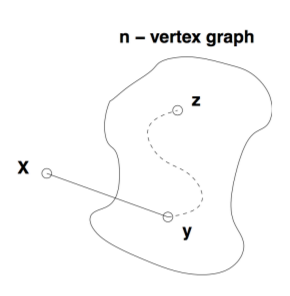
\includegraphics{build_up_error}
\centering
\end{figure}
 
\end{proof}


\begin{questions}
\question Give a counter-example to show the claim is false.

\begin{solution} [1 in]
Consider 2 pairs of vertices where each pair is connected by an edge. Each vertex has degree 1 but the two pairs are distinct connected components and the graph is disconnected.
\end{solution}

\question Since the claim is false, there must be an error in the proof. Explain the error. 
\begin{solution} [1 in]
The proof is actually logically correct until the last sentence. The problem is that for $P(n+1)$ to be true, we must show that every ($n+1$)-vertex positive-degree graph is connected. Instead, the proof shows that every ($n+1$)-vertex positive-degree graph that can be constructed by adding a vertex of positive degree to an existing ($n$)-vertex positive-degree graph. Confirm that there is no way to build your counter-example graph by the method in the proof. 

More generally, this is an example of "build-up error". This error arises from a faulty assumption that every graph of size $n+1$ with some property can be built by adding a vertex to an $n$ vertex graph that also has that property. This assumption is correct in some cases, and incorrect in others. 

In this class you will most likely only see build-up error in graph problems, but its important to understand that this can occur anytime you are doing induction on the size of some mathematical structure (i.e. matrices). 

\end{solution}

\question How can we avoid this mistake?
\begin{solution} [1 in]
We want to consider all possible ($n+1$)-vertex graphs but we also want to apply our induction hypothesis. The correct way to do this is to use a "shrink down, grow back" approach where we start with a graph on $n+1$ vertices that we assume satisfies the property we care about, remove an arbitrary vertex, and show that the induction hypothesis still holds for the new graph. Then add back the vertex and argue that $P(n+1)$ holds. 
\end{solution}

\question What happens in the inductive step when you apply the fix?
\begin{solution} [1 in]
Consider a graph on $n+1$ vertices where every vertex has degree at least $1$. Remove an arbitrary vertex leaving an $n$-vertex graph. To apply the inductive hypothesis to this graph, we need every vertex to have positive degree, but this is not guaranteed to happen when we remove an arbitrary vertex. Thus we are stuck, unable to apply the inductive hypothesis.
\end{solution}
\end{questions}


% \begin{solution}
% Build up error! Always start with the $n+1$ case, \textbf{especially} 
% when working with graphs. If we start with a graph that has $n+1$ 
% vertices, is it possible to work with such a graph that removing one 
% vertex will create a graph with $n$ vertices, but which is disconnected?
% \end{solution}

\clearpage